\documentclass{standalone}
\usepackage{tikz}
\begin{document}
% TI-84 Plus CE CALC ZERO screen; 1 unit = 1 screen pixel of the 244x184 screenshot
% Graph window measured from the pixels: x in [0,6] (Xscl 1), y in [0,25] (Yscl 1)
\newcommand{\tineg}{\raisebox{0.55ex}{\fontsize{5}{5}\selectfont-}}
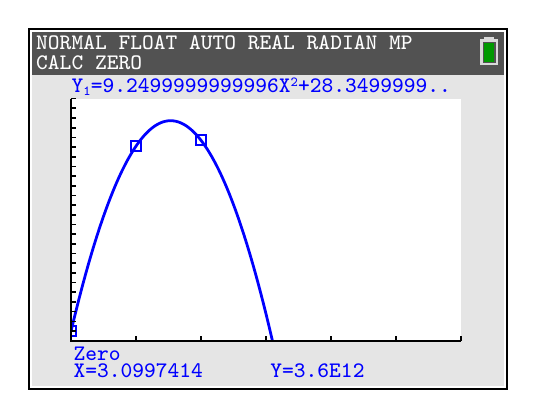
\begin{tikzpicture}[x=0.025cm, y=-0.025cm,
    every node/.style={inner sep=0pt, font=\ttfamily\bfseries\fontsize{7.8}{9}\selectfont},
    status/.style={anchor=west, text=white, font=\ttfamily\bfseries\fontsize{8}{9}\selectfont}]
  % Screen background
  \fill[black!10] (0,0) rectangle (244,184);
  % Status bar
  \fill[black!68] (2,2) rectangle (242,24);
  \node[status] at (4,7.5)  {NORMAL FLOAT AUTO REAL RADIAN MP};
  \node[status] at (4,17.5) {CALC ZERO};
  % Battery icon (full)
  \draw[black!15, line width=0.8pt] (230.5,6.5) rectangle (238.5,18.5);
  \fill[black!15] (232,4.5) rectangle (237,6);
  \fill[green!60!black] (232,7.5) rectangle (237,17.5);
  % Equation line (truncated on screen)
  \node[anchor=west, text=blue] at (22,30)
    {Y\raisebox{-0.35ex}{\fontsize{5}{5}\selectfont 1}=\tineg9.2499999999996X\raisebox{0.6ex}{\fontsize{5}{5}\selectfont 2}+28.3499999..};
  % Graph window: x-axis along the bottom (y=0), y-axis along the left edge (x=0)
  \fill[white] (22,36) rectangle (220,159);
  \begin{scope}
    \clip (22,36) rectangle (220,159);
    % Y1 = -9.2499999999996x^2 + 28.3499999...x + c; c is cut off on screen,
    % c = 1 makes the zero land at the displayed X=3.0997414 and matches the pixels
    \draw[blue, line width=1pt, smooth, samples=150, domain=0:3.2]
      plot ({22+33*\x}, {159-4.92*(-9.25*\x*\x + 28.35*\x + 1)});
    % Square plot markers (y read from pixel positions; the one at x=0 is mostly clipped)
    \foreach \px/\py in {0/1, 1/20.1, 2/20.7}
      \draw[blue, line width=0.8pt] ({22+33*\px-2.5}, {159-4.92*\py-2.5})
        rectangle ++(5,5);
  \end{scope}
  % Axes with unit tick marks
  \draw[black, line width=0.8pt] (22,36) -- (22,159) -- (220,159);
  \foreach \t in {1,...,5}
    \draw[black, line width=0.6pt] ({22+33*\t},159) -- ({22+33*\t},156.5);
  \draw[black, line width=0.6pt] (220,159) -- (220,156.5);
  \foreach \t in {1,...,25}
    \draw[black, line width=0.6pt] (22,{159-4.92*\t}) -- (24.5,{159-4.92*\t});
  % Result readout
  \node[anchor=west, text=blue] at (23,165.5) {Zero};
  \node[anchor=west, text=blue] at (23,174.5) {X=3.0997414};
  \node[anchor=west, text=blue] at (123,174.5) {Y=\tineg3.6E\tineg12};
  % Outer screen border
  \draw[white, line width=1pt] (1.5,1.5) rectangle (242.5,182.5);
  \draw[black, line width=0.8pt] (0.5,0.5) rectangle (243.5,183.5);
\end{tikzpicture}
\end{document}
